\chapter{État de l'art des techniques}
\chaptermark{Techniques}
\minitoc
\newpage
 
\section{État de l'art des techniques classiques}
Pour pouvoir affecter une transaction à un magasin ou identifier son origine, il existe plusieurs procédés permettant de résoudre ce problème. Pour cela nous ferons le parcours des meilleurs algorithmes utilisés comme Store locator, Alpha / Alpha City et Patterns regex.

\subsection{Store Locator:}
\begin{itemize}
\item Contexte:\\
Store Locator vise à enrichir les transactions qui respectent les critères suivantes:
\\
- Présence du nom du magasin dans lequel la transaction a été effectuée (identifiant du magasin). L'idée derrière cet algorithme est que si nous savons qu'il n'y a qu'un seul magasin d'un détaillant dans une zone géographique et si nous sommes capables de détecter cette zone géographique et que le nom du détaillant se trouve dans le label de transaction (“CB CARREFOUR 045 02/03/2021 10€”), nous pouvons l'attribuer à ce magasin spécifique.\\
- Présence de la ville dans laquelle la transaction a été effectuée (identifiant de la ville).\\
- S'il n'a pas été possible d'associer la transaction à un magasin, déterminer s'il s'agit d'une transaction hors centre commercial, c'est-à-dire hors du centre commercial dans lequel le client est enregistré.
\item Notion de zone géographique:\\
Tout d’abord on crée toutes les zones géographiques de manière hiérarchique sous forme d’un arbre n-aire avec une relation de parent à fils et à la racine le monde. Le centre commercial est placé comme étant fils de la ville  (ex: Les 4 Temps dans la ville de Puteaux). Cette configuration permet de faire un parcours de manière hiérarchique en base à la recherche de la zone géographique correspondante à une transaction.
\newpage
\begin{figure}[h]
\begin{center}
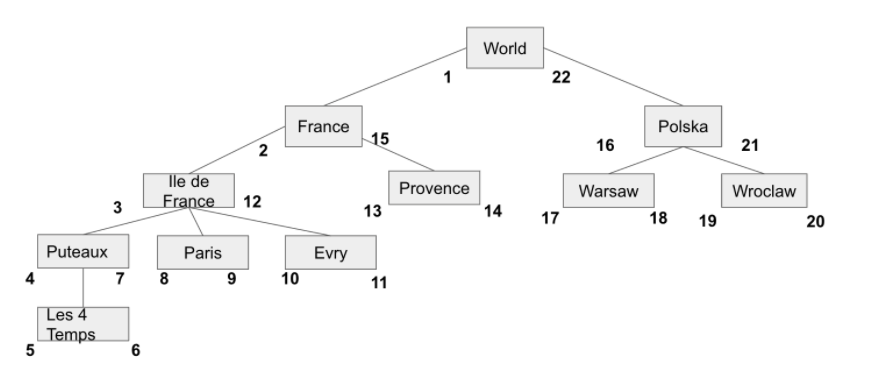
\includegraphics[width=15cm,height=8cm]{images/tree_geographical.png}
\caption[Arbre des zones géographiques]{Arbre des zones géographiques}
\label{monlabel}
\end{center}
\end{figure}
\item Affectation ou correspondance:\\
La première étape consiste à trouver si les transactions ont un pattern correspondant.
\item Correspondance des zones géographiques:\\ 
Pour attribuer une transaction à un magasin ou à une ville, nous devons d'abord connaître sa zone géographique. Pour chaque pattern de zone géographique en base, on recherche les transactions qui correspondent à ce pattern. \\
- Affectation de la ville et du magasin:\\
Une fois la correspondance effectuée, nous pouvons procéder aux affectations. Lorsqu'on n'est pas en mesure d'associer la transaction à un magasin, on veut au moins savoir si elle a été effectuée en dehors du centre commercial. On rappelle qu’ une transaction peut potentiellement être considérée comme hors centre commercial en fonction des valeurs du détaillant et de la zone géographique dans la matrice ci-dessous.
\newpage 
\begin{figure}[h]
\begin{center}
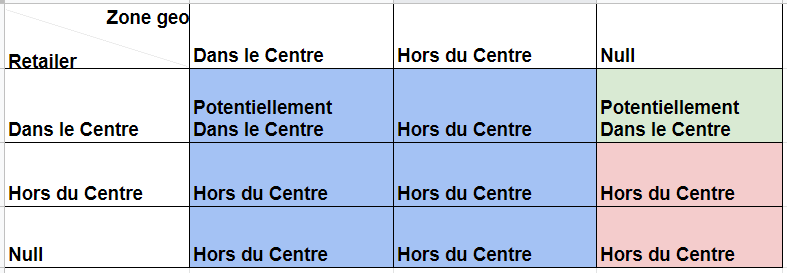
\includegraphics[width=15cm,height=6cm]{images/inmall_outmall.png}
\caption[Règle d'affectation des transaction dans le centre et en déhors]{Arbre des zones géographiques}
\label{monlabel}
\end{center}
\end{figure}


 Les transactions passent par différents processus en fonction de leur zone géographique et de la valeur des détaillants :
\begin{itemize}
\item Transactions en bleu : \\
Pour les transactions dont leur zone géographique est non nul on garde celle qui matche avec des patterns de zone géographique 
    - On regroupe les transactions suivant leur patterns de zone géographique afin d'avoir pour chaque ensemble la zone géographique liés à l'ensemble des transactions qu'ils ont appariées.\\
    - Pour chaque ensemble de zones géographiques, nous voulons d'abord réduire l'ensemble des zones géographiques potentielles aux plus discriminantes si l'ensemble des zones géographiques potentielles est composé de plusieurs zones. Les zones géographiques sont organisées sous forme de hiérarchie. Ainsi, si une zone géographique contient une autre zone géographique, nous conservons la zone géographique au niveau le plus bas. À ce stade, il peut encore y avoir plusieurs zones géographiques potentielles.\\
    - Après cette première présélection, nous choisissons les magasins qui se trouvent dans l'ensemble réduit de zones géographiques.\\
    - Une fois que nous avons la liste des magasins potentiels, nous voulons savoir si nous pouvons attribuer la transaction à un magasin unique.
\newpage

Pour chaque zone géographique de la liste des magasins potentiels, nous regardons s'il n'y a qu'un seul magasin dans la zone géographique. Si à la fin il n'y a qu'un seul magasin, nous pouvons attribuer nos transactions à ce magasin unique et à la ville correspondant à ce magasin. 

        Si nous ne sommes pas en mesure d'attribuer nos transactions à un magasin, nous essayons de l'attribuer à une ville. Le processus est le même que pour les magasins mais nous regardons dans la liste des zones géographiques potentielles. 

    Pour les transactions que nous n'avons pas réussi à attribuer à un magasin, nous voulons au moins préciser si elles étaient en dehors du centre commercial. 

\item Transaction en jaune:\\
Ces transactions n’ont pas de zone géographique connue mais ont un détaillant dans le centre commercial connu. Elles peuvent être potentiellement dans le centre. 

\item Transactions en rouge:\\
Ces transactions n’ont pas de zone géographique connue et le détaillant n’est non plus connu ou sont hors du centre où le client est enregistré. On peut conclure que ces transactions sont effectuées en dehors du centre du client.

\end{itemize}
\end{itemize}
\newpage
\subsection{Alpha:}
Alpha est un algorithme qui prend en entrée le label de la transaction, effectue une requête à l'API des lieux de Google, et si l'API renvoie un seul résultat et si ce résultat est de type détaillant, il attribue le magasin à la transaction. Afin d'éviter de créer des doublons de magasins, nous utilisons l'identifiant de google appelé google-place-id (ex: ChIJo82pu26q2EcRRvXT8RUamHo) retourné.\\
De plus, afin d'éviter de faire la même requête à google à chaque fois, lorsque la requête a été postée, elle est stockée dans une table en base.
Pour chaque requête, on vérifie d'abord dans cette table pour éviter tout coût supplémentaire.

\subsection{Alpha City:}
Alpha city est une évolution d'alpha où au lieu d'interroger le label de transaction à l'API google de lieux, la requête est de la forme nom-détaillant + ville (donc on doit avoir détecté une ville et un détaillant dans le label pour pouvoir faire une requête). A part cela, le mécanisme est exactement le même que celui d'Alpha.

Détection de la ville:
Afin de détecter la ville dans le label, une façon de procéder est d'utiliser des mots-clés. Cette méthode a l'avantage d'être très précise si les mots-clés sont bien conçus mais l'inconvénient est de ne pas être évolutive du tout: si on veut détecter n'importe quelle ville dans le monde, on doit déclarer des mots-clés pour chaque ville. C'est pourquoi les mots-clés sont utilisés pour la localisation des magasins (lorsque le but est d'attribuer une transaction à l'intérieur du centre et que toute erreur peut conduire à une récompense cliente inappropriée). 

Pour la détection de masse des villes, la méthode consiste à calculer la distance de Levenshtein entre le label des transactions et les villes. De manière informelle, la distance de Levenshtein entre deux mots est le nombre minimum de modifications d'un seul caractère (insertions, suppressions ou substitutions) nécessaires pour transformer un mot en l'autre. Si la distance entre le label et la ville est suffisamment faible, l'algorithme attribue la ville à la transaction.

La distance de Levenshtein entre deux cordes $a, b$ un B (de longueur $|a|$ et $|b|$ respectivement) est donnée par ${lev} (a,b)$ où

\begin{figure}[h]
\begin{center}
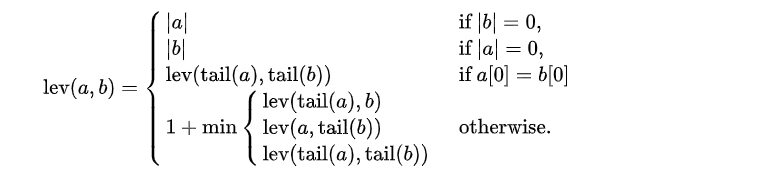
\includegraphics[width=15cm,height=3.5cm]{images/distance_levenshtein.png}
\label{monlabel}
\end{center}
\end{figure}

\newpage
\section{Etat de l’art des algorithmes de machine learning}

\subsection{Méthode de Support Vector Machine SVM:}
D’après l’article Proposé par Boser, Guyon, et Vapnik en 1992, SVM est une technique de classification linéaire et non linéaire.
SVM est un modèle d’apprentissage supervisé basé sur la détermination d’un hyperplan qui sépare les données d’une classe des autres classes.
\begin{figure}[h]
\begin{center}
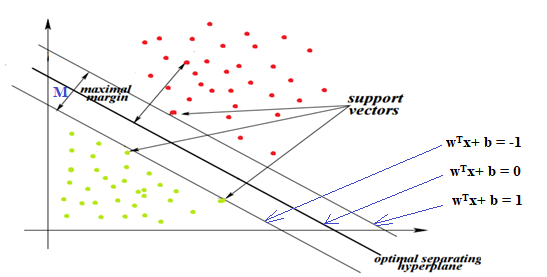
\includegraphics[width=15cm,height=8cm]{images/svm_separate.png}
\caption[Hyperplan de séparaton des points de données]{Hyperplan de séparaton des points de données}
\label{monlabel}
\end{center}
\end{figure}


\begin{figure}[h]
\begin{center}
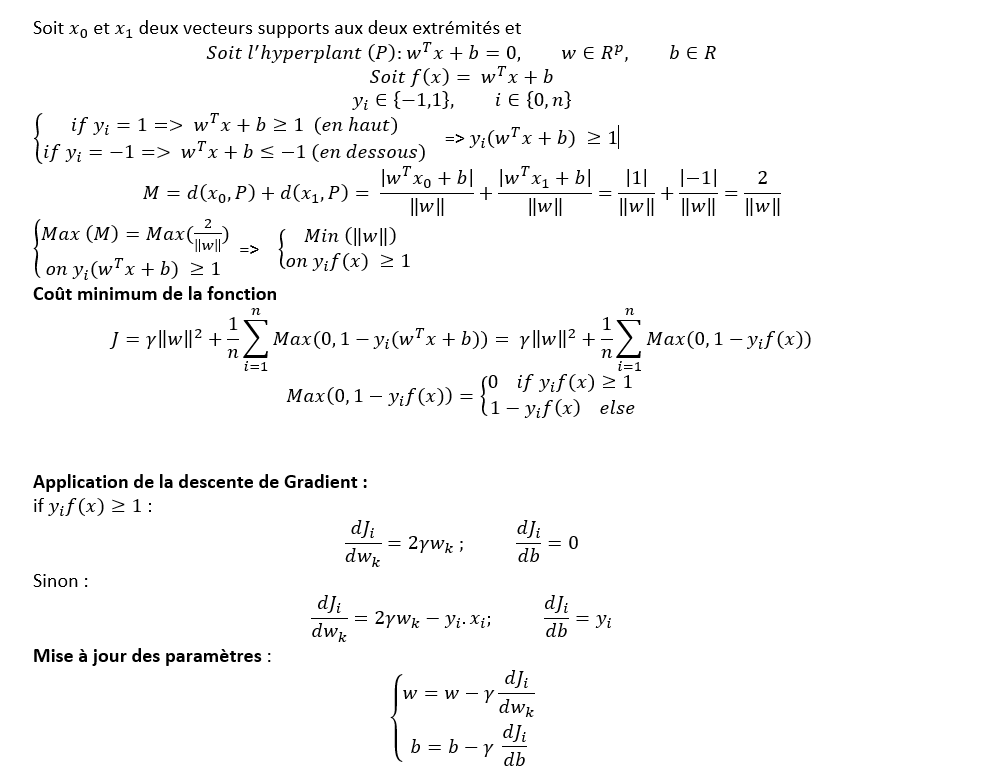
\includegraphics[width=15cm,height=13cm]{images/svm_equation.png}

\label{monlabel}
\end{center}
\end{figure}
\newpage

\subsection{Méthode du Decision tree:}
L'apprentissage par arbre de décision ou induction d'arbres de décision est l'une des approches de modélisation prédictive utilisées en statistique, en exploration de données et en apprentissage automatique. Elle utilise un arbre de décision pour passer des observations sur un élément aux conclusions sur la valeur cible de l'élément.
Considérons l’exemple dans lequel on souhaite construire l’arbre de décision sur une donnée pouvant prévoir le moment idéal de sortir en fonction de la météo. Pour chaque nœud , la règle consiste à trouver la meilleure colonne (ex: Time) et le séparateur idéal sur cette colonne (ex: Time > 10 ?)\\
\begin{figure}[h]
\begin{center}
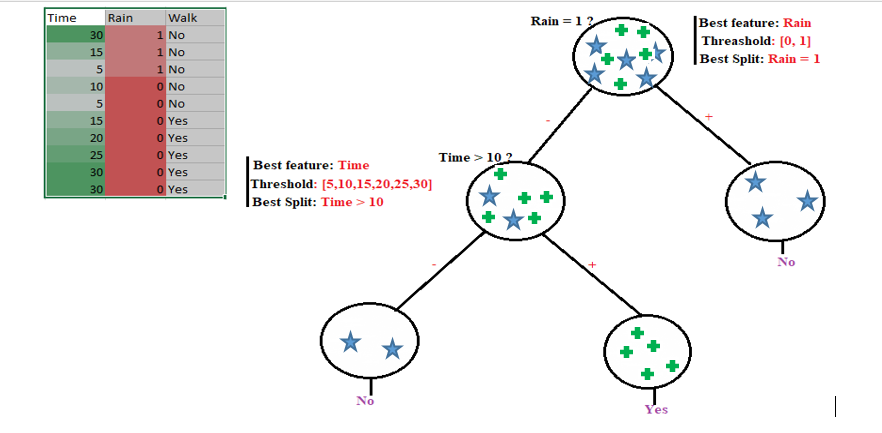
\includegraphics[width=15cm,height=8cm]{images/decision_tree_formular.png}
\caption[Arbre de décision]{Arbre de décision}
\label{monlabel}
\end{center}
\end{figure}
On choisit le meilleur feature et le meilleur threshold en se basant sur le calcul du gain d’information à partir de l’entropie ou le gini de l’information. On construit donc les fils du nœud en faisant la séparation à partir de la meilleure coupure (Best Split). Au bout de la profondeur de l’arbre fixée, la décision dans chaque feuille est la classe avec une majorité de données.
\newpage
\begin{figure}[h]
\begin{center}
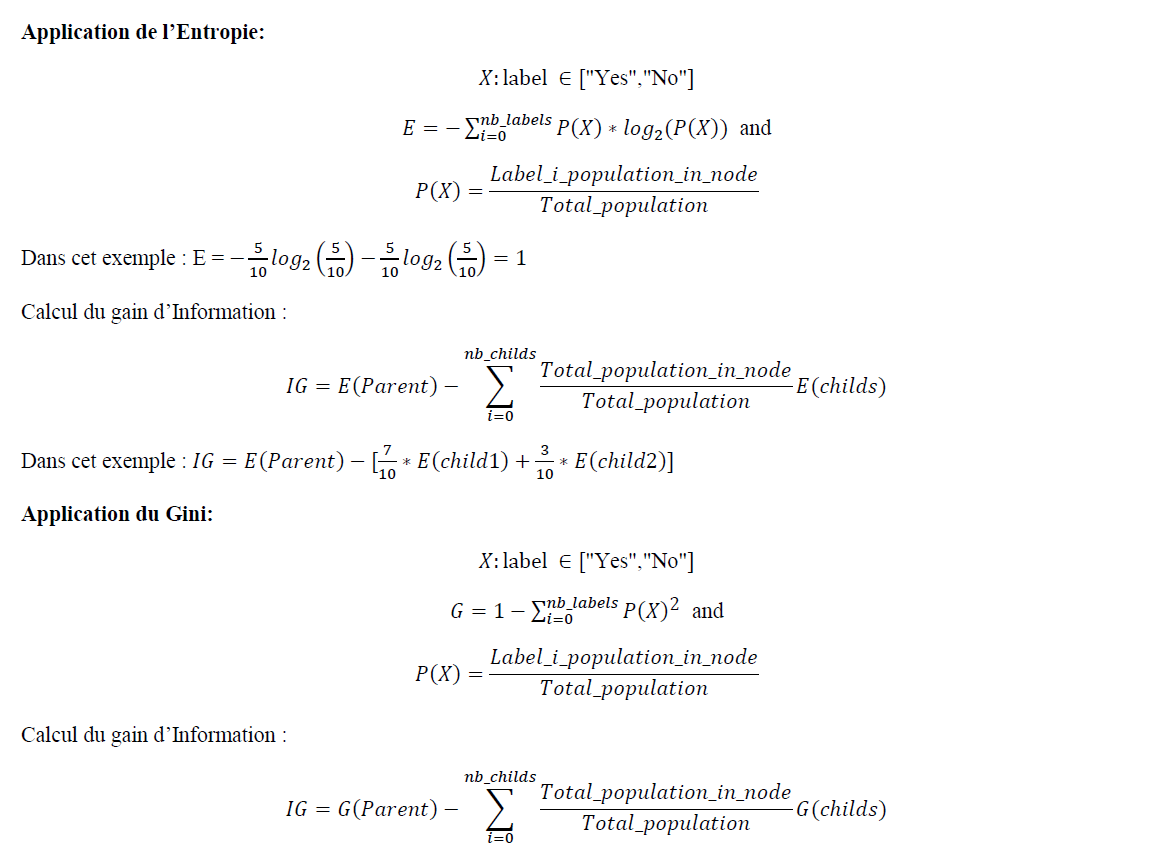
\includegraphics[width=15cm,height=12cm]{images/decision_tree_equation.png}
\label{monlabel}
\end{center}
\end{figure}
\newpage

\subsection{Méthode du Random Forest:}
Le random forest un algorithme de classification supervisé basé sur la combinaison de plusieurs arbres N de décision appelés Décision Tree. Comme définie dans [3]  chaque arbre décisionnel est réalisé en sélectionnant aléatoirement les données parmi les données disponibles. Par exemple, une forêt aléatoire pour chaque arbre décisionnel peut être construite par l'échantillonnage aléatoire d'un sous-ensemble de caractéristiques, et/ou par l'échantillonnage aléatoire d'un sous-ensemble de données d'entraînement pour chaque arbre décisionnel.
\begin{figure}[h]
\begin{center}
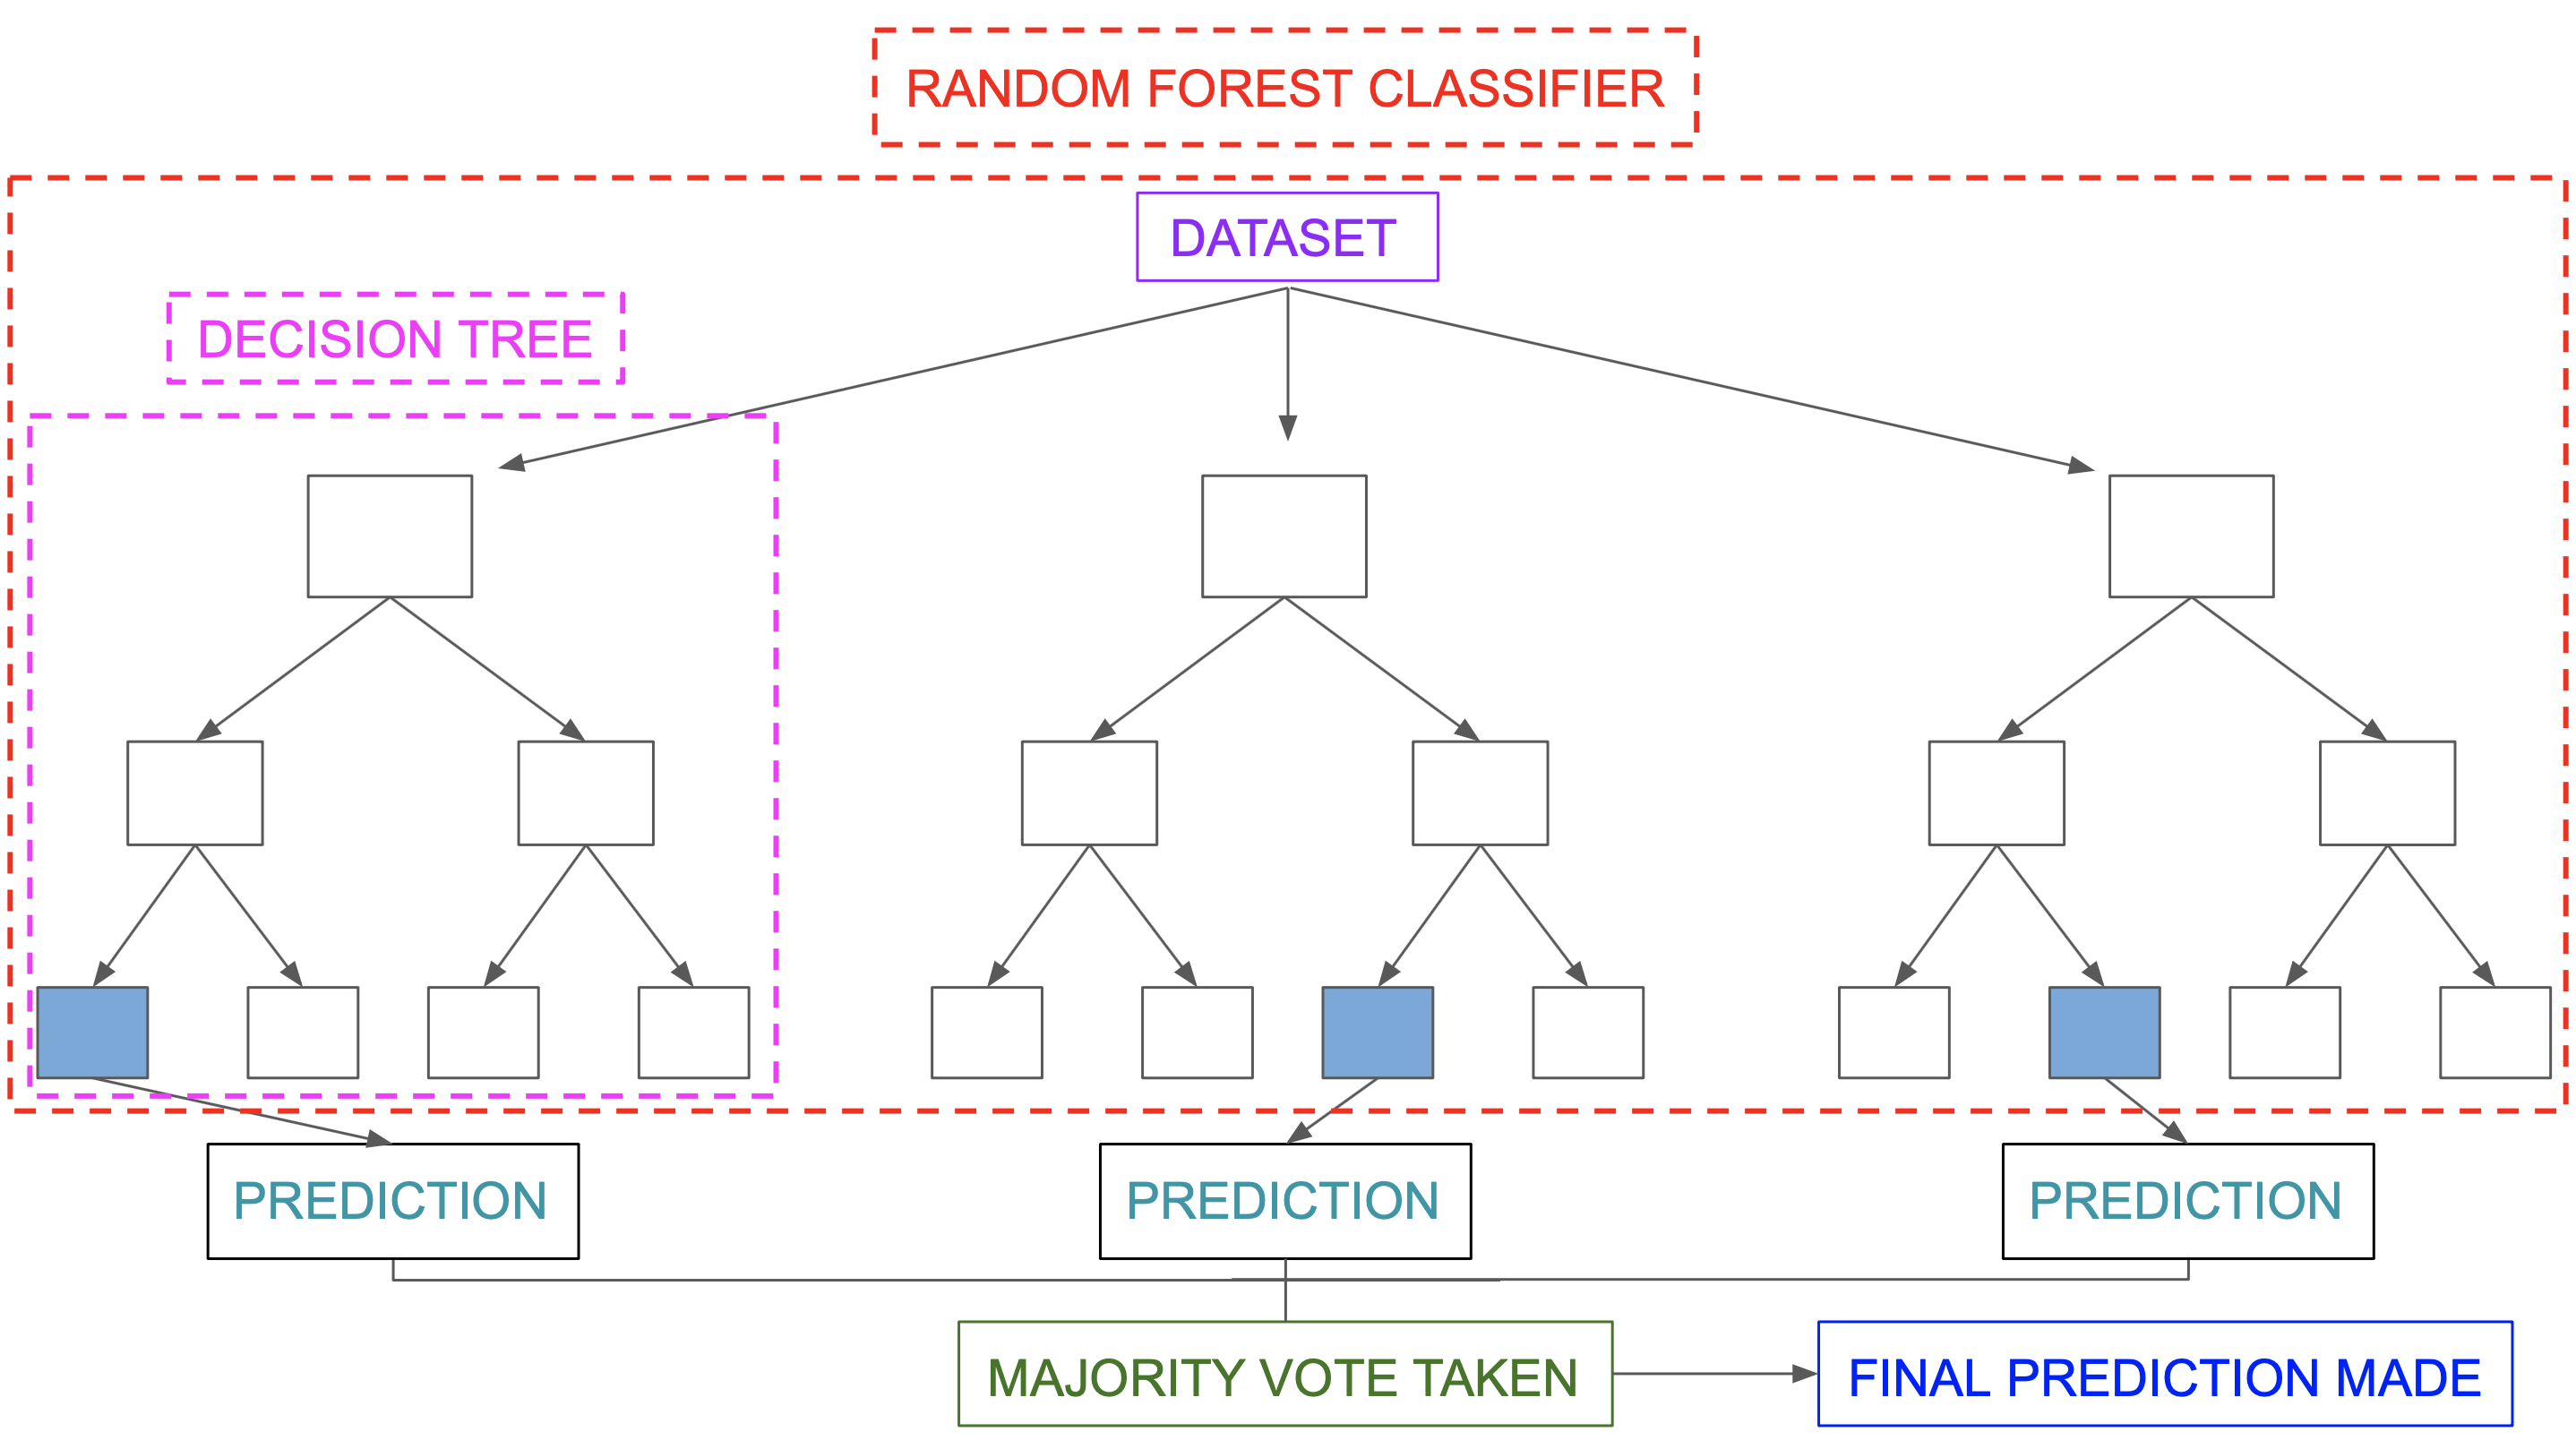
\includegraphics[width=15cm,height=9cm]{images/random-forest-classifier.png}
\caption[Foret aléatoire]{Foret aléatoire}
\label{monlabel}
\end{center}
\end{figure}
Pour avoir la décision finale, on calcule la moyenne des décisions prises par l’ensemble des arbres de décision de la forêt.
\newpage


\subsection{K- Nearest Neighbor}
\begin{figure}[h]
\begin{center}
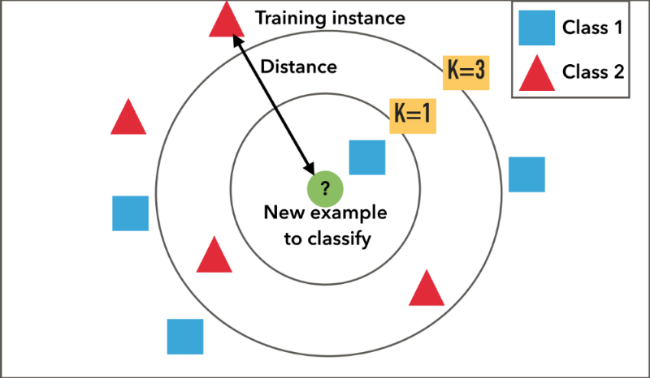
\includegraphics[width=15cm,height=8cm]{images/knn_sheama.png}
\caption[K- Nearest Neighbor]{K- Nearest Neighbor}
\label{monlabel}
\end{center}
\end{figure}
\begin{enumerate}
\item Pricipe du K- Nearest Neighbor:\\
Le K-Nearest Neighbor est un algorithme de machine learning d’apprentissage supervisé qui a pour principe de déterminer les K premiers points de données les plus proches en termes de distance par rapport à un point de donnée. 
\item Les types de distances:\\
On distingue différentes sortes de distances applicable au KNN:
\begin{itemize}
		\item Distance euclidienne
		$$d(A,X) = \sqrt{\sum_{i=1}^{n} (a_{i}-x_{i})^{2}}$$
		\item Distance de Manhattan\\
		$$d(A,X) = \sum_{i=1}^{n} \mid{a_{i}-x_{i}}\mid$$
		\item Distance de Minkowski
		$$d(A,X) = \sqrt[p]{\sum_{i=1}^{n} \mid{a_{i}-x_{i}}\mid^{p}}$$
\end{itemize}
\item Choix du paramètre K:
\begin{itemize}
		\item Utilisation de K
		Le choix du paramètre K peut être effectué en prenant la partie entière de la racine carré du nombre de jeu de donnée 
		$$K=\sqrt{nombre-de-donnees }$$
		\item Choisir K suivant celui qui donne une meilleure prédiction:\\		
		La meilleure valeur de K est aussi déterminée en faisant des tests sur différentes valeurs de K.
\end{itemize}
\end{enumerate}
